\documentclass[
    oneside,
    ngerman,
    footinclude=false,
    captions=tableheading,
    DIV=12
]{scrartcl}


\usepackage{UniLaTeXPackage}

\ihead{Tom Folgmann,\\David Jannack}
\chead{Daniel Kazenwadel\\Blatt 04}
\ohead{\today}

\begin{document}
\aufgabe{}
\subaufgabe{}
    Sei die Kraft auf ein Teilchen durch die Funktion
    \[F_s:=\fdef{\sum_{i\in[s]}\frac{1}{\dabs{r - R_i}{2}^3}\cdot (r-R_i)}{r\in\R^3}\]
    gegeben, wobei $R$ das \emph{Magnetorttupel} mit Vektoren $R_i\in\R^3$ ist. Die Bewegungsgleichung ist dann gegeben durch $m\cdot r''(t) = (F_s\circ r)(t)$. Für $s = 3$ erhalten wir die mit der Masse $m$ angepasste rechte Seite $F$ aus Beschleunigung des Pendels mit der Definition
    \[f:=\fdef{\frac{1}{m}\cdot\sum_{i\in[3]}\frac{x-R_i}{\dabs{x-R_i}{2}^3}}{(t,x)\in D_1},\]
    wobei wir $D_n:=\R\times(\R^3)^n$ abkürzen. Die Reduktion der Ordnung ergibt
    \[v(t):=\begin{pmatrix}
        x(t)\\x'(t)
    \end{pmatrix},\quad v'(t)=\begin{pmatrix}
        v_2^*(t)\\f(t,v_1^*(t))
    \end{pmatrix}.\]
    Damit ergibt sich die vektorwertige rechte Seite
    \[F:=\fdef{\begin{pmatrix}
        x_2\\f(t,x_1)
    \end{pmatrix}}{(t,x)\in D_2}\implies F(t,(x(t),x'(t))) = \begin{pmatrix}
        x'(t)\\\frac{1}{m}\cdot\sum_{i\in[3]}\frac{x(t)-R_i}{\dabs{x(t)-R_i}{2}^3}
    \end{pmatrix}\]
    für eine Lösung $x:\R\to \R^3$. Im Reibungs- und Federfall erweitere $f$ derart, daß beide berücksichtigt werden:
    \[\tilde f:=\fdef{\frac{1}{m}\cdot \nbra{F_s(t,x_1) - \gamma\cdot x_2 - k\cdot x_1}}{(t,x)\in D_2}.\]
    Damit ergibt sich die neue rechte Seite
    \[\tilde F:=\fdef{\begin{pmatrix}
        x_1\\\tilde f(t,x_1)
    \end{pmatrix}}{(t,x)\in D_2}.\]

\subaufgabe{}
    Für die Magnetpositionen wählen wir den Einheitskreis um $0_{\R^2}$ gemäß $\mcK_{1,0_{\R^2}}(x):=\bbra{\Phi({\exp}(\cmath\cdot\varphi))}_{\varphi\in(-\pi,\pi)}$ für $\Phi:=\bbra{\Real(z),\Imag(z)}_{z\in\C}$ als Konstruktionsfunktion. Um den Masseschwerpunkt in den Ursprung $(0,0)$ zu legen, Zerlegen wir $(-\pi,\pi)$ in Intervalle gleichen Durchmessers und finden $\varphi_1:=0$, $\varphi_2:=\pi/3$ und $\varphi_3:=-\pi/3$. Somit ist das Magnetorttupel gegeben durch
    \[
        R:=\Big(\big(\cos(\varphi_i),\sin(\varphi_i)\big)\Big)_{i\in[3]}.
    \]
    Damit ergeben sich konkret die Orte $R_1 = (0,1)$, $R_2 = (\sqrt{3}/2,-1/2)$ und $R_3 = (-\sqrt{3}/2,-1/2)$ und somit die folgende optische Verteilung:
    \begin{figure}[H]
        \centering
        \begin{tikzpicture}
            \draw[->] (-1.5,0) -- (1.5,0) node[right] {$x$};
            \draw[->] (0,-1.5) -- (0,1.5) node[above] {$y$};

            \draw[loosely dotted] (0,0) circle (1cm);

            \draw[red,->] (0,0) -- (0,1) node[above left] {$R_1$};
            \draw[red,->] (0,0) -- (0.866,-0.5) node[below right] {$R_2$};
            \draw[red,->] (0,0) -- (-0.866,-0.5) node[below left] {$R_3$};
        \end{tikzpicture}
        \caption{Magnetorttupel im $\R^2$ Anschauungsraum.}
    \end{figure}


\subaufgabe{}
    Wir verwenden die bestimmten Gleichungen gemäß Aufgabenteil (a) in Kombination mit dem Lösungsalgorithmus \enquote{Leap Frog} und \enquote{Velocity Verlet}. 

\subaufgabe{}
    \textbf{Die Implementierung ist unter $\to$\href{https://github.com/unb3rechenbar/ComputerPhysik-I-Projekte.git}{Github} im Ordner \enquote{Blatt 04 - Projekt 2 (Magnetpendel)/Simulation} unter dem im Readme angegebenen Abgabecommit vorzufinden}. Wir erzeugen dabei eine Tabelle mit den Spalten $t,u_x(t),u_y(t),u'_x(t),u'_y(t)$. 

\subaufgabe{}
    Drei Beispieltrajektorien sind die folgenden. Wir verwenden $\gamma = 0.2$ und $k = 0.05$. 
    \begin{figure}[H]
        \centering
        \includegraphics[width=10cm]{../Simulation/img/trcs/velverl3-0-0-0-0.png}
        \caption{Anfangsbedingungen $u(0) = (0,0)$ und $u'(0) = (0,0)$.}
    \end{figure}

    \begin{figure}[H]
        \centering
        \includegraphics[width=10cm]{../Simulation/img/trcs/velverl3-314-314-0-0.png}
        \caption{Anfangsbedingungen $u(0) = (\pi,\pi)$ und $u'(0) = (0,0)$.}
    \end{figure}

    \begin{figure}[H]
        \centering
        \includegraphics[width=10cm]{../Simulation/img/trcs/velverl3-0-1.5--15-0.png}
        \caption{Anfangsbedingungen $u(0) = (0,1.5)$ und $u'(0) = (-15,0)$.}
    \end{figure}

    Wir mussten dabei die Magnetkraft mit einem konstanten Faktor $3$ multiplizieren, da die Wirkung der Pfade durch den hohen Magnetabstand sonst nicht zur Gältung käme. 

\subaufgabe{}
    Wir erhalten für den Farbplot die folgende Abbildung. 
    \begin{figure}[H]
        \centering
        \includegraphics[width=7cm]{../Simulation/img/Farbbild-k=05.png}
        \caption{Farbplot der Konvergenzen bei $k = 0.5$ und $\gamma = 0.2$.}
    \end{figure}
    Die Abbildung zeigt den Bereich $[-6,6]\times[-6,6]$ bei einer Auflösung von $200$ Punkten pro Kante um den Nullpunkt. Die drei Magnete befinden sich an den in (b) bestimmten Orten. Für eine Federkonstante $k = 0.05$ erhalten wir folgende. 
    \begin{figure}[H]
        \centering
        \includegraphics[width=7cm]{../Simulation/img/Farbbild-k=005.png}
        \caption{Farbplot der Konvergenzen bei $k = 0.05$ und $\gamma = 0.2$.}
    \end{figure}
    Man kann im Übrigen auch sehr schön betrachten, wie mit variierender Reibungskonstante $\gamma$ die Konvergenz sich verändert und zunehmend chaotisch wird:
    \begin{figure}[H]
        \begin{subfigure}[b]{0.49\textwidth}
            \centering
            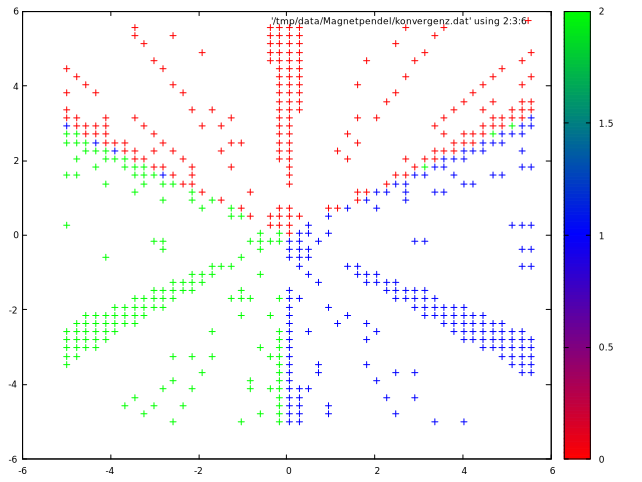
\includegraphics[width=7cm]{../Simulation/img/Farbbild-g1.png}
            \caption{$\gamma = 1$.}
        \end{subfigure}
        \begin{subfigure}[b]{0.49\textwidth}
            \centering
            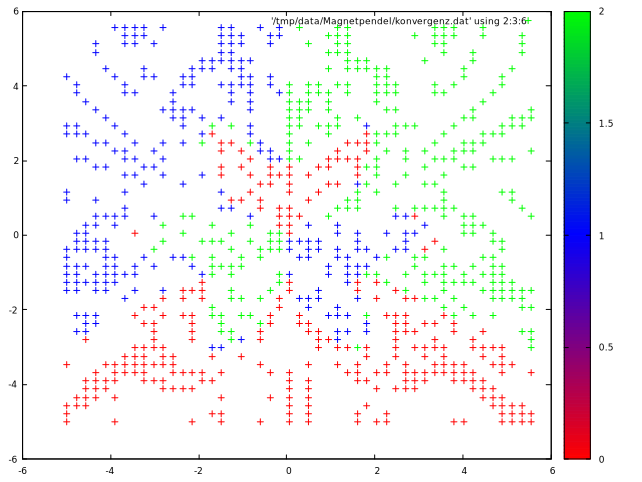
\includegraphics[width=7cm]{../Simulation/img/Farbbild-g05.png}
            \caption{$\gamma = 0.5$.}
        \end{subfigure}
        \begin{subfigure}[b]{0.49\textwidth}
            \centering
            \includegraphics[width=7cm]{../Simulation/img/Farbbild-g01.png}
            \caption{$\gamma = 0.1$.}
        \end{subfigure}
        \begin{subfigure}[b]{0.49\textwidth}
            \centering
            \includegraphics[width=7cm]{../Simulation/img/Farbbild-g001.png}
            \caption{$\gamma = 0.01$.}
        \end{subfigure}
        \caption{Farbplots der Konvergenzen bei $k = 0.05$ und $\gamma = 1,0.5,0.1,0.01$.}
    \end{figure}

\subaufgabe{}
    Für mehrere Magneten variiere $s$ und berechne die neuen Magnetorte auf dem Einheitskreis durch 
    \[
        R:=\fdef{\nbra{\cos(\frac{n\cdot \pi}{s - 1}),\sin(\frac{n\cdot pi}{s - 1})}}{n\in\{0,\dots,s-1\}}.
    \]
    Wir erhalten für vier Magneten das folgende Bild:
    \begin{figure}[H]
        \centering
        \includegraphics[width=7cm]{../Simulation/img/Farbbild-4Mag0502.png}
        \caption{Farbplot der Konvergenzen bei $k = 0.05$, $\gamma = 0.2$ und $s = 4$.}
    \end{figure}
    Für zwei Magneten erhalten wir weiter das folgende Bild.
    \begin{figure}[H]
        \centering
        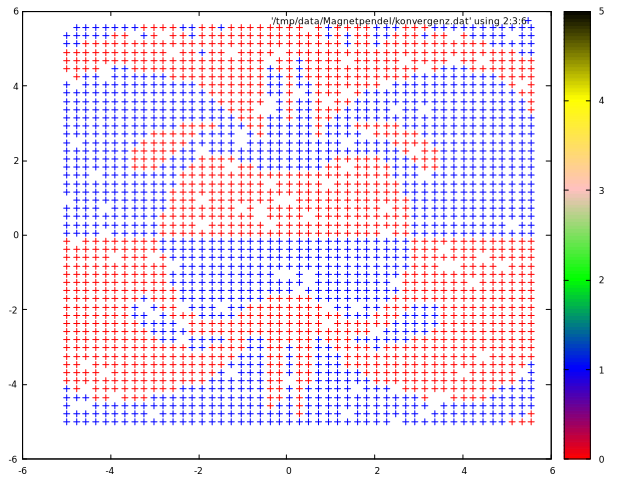
\includegraphics[width=7cm]{../Simulation/img/Farbbild-2Mag0502.png}
        \caption{Farbplot der Konvergenzen bei $k = 0.05$, $\gamma = 0.2$ und $s = 2$.}
    \end{figure}
    Für ein Vielmagnetensystem mit beispielsweise $s = 6$ Instanzen wird das Bild jedoch lückenhaft, da in den gegebenen Bereichen $T = 200$, $h = 0.001$ und $r_\textit{min} = 0.001$ keine Lösungen gefunden werden können. Dies führt zu folgender Grafik.
    \begin{figure}[H]
        \centering
        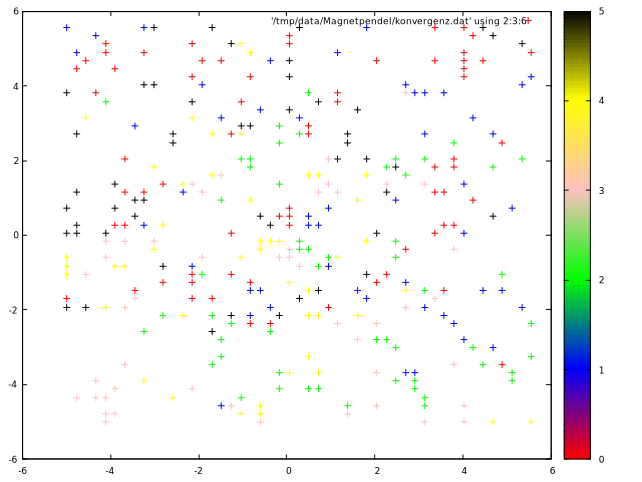
\includegraphics[width=7cm]{../Simulation/img/Farbbild-6Mag0502.png}
        \caption{Farbplot der Konvergenzen bei $k = 0.05$, $\gamma = 0.2$ und $s = 6$.}
    \end{figure}
    Hier könnte Parallelisierung der Prozesse und Optimierung des Codes mit längerer Laufzeit abhilfe schaffen - Bart gab sein bestes. 

\end{document}
